\newcommand{\ClassPath}{../../yukibook.cls}
\documentclass{\ClassPath/yukibook}


\begin{document}

    \yukibook{Sistemas de control de versiones} % Title
    {Rubén Gómez Olivencia}  % Author
    {2023}    % Year
    {} % Name of degree
    {Si no usas uno, no eres programador} % catch phrase
    {} % the phrase's author
    {img/git.png} %cover
    {3d2d00}
    {} %mini-title

        \coverpage
        \graphicspath{{../../yukibook.cls/}}
        \licensepage
    %
        \tableofcontents

    %--------------------------------------------------------------------------
    % Start your parts, chapters and sections here
    %--------------------------------------------------------------------------
    \graphicspath{{img/}}
    \part{Sistemas de control de versiones}
    \chapter{Introducción}

Un sistema de control de versiones es un sistema que nos permite tener un histórico de las modificaciones que sufre un fichero a lo largo del tiempo.

Si pensamos en un documento, un ciclo de vida con modificaciones puede ser:

\begin{enumerate}
    \item Crear el documento.
    \item Correcciones.
    \item Cambios gramaticales.
    \item Modificar colores de los encabezados.
    \item Añadir logo de la compañía.
    \item Modificaciones finales.
\end{enumerate}

Los sistemas de control de versiones pueden controlar las modificaciones de cualquier tipo de fichero, pero son especialmente útiles cuando se trata con ficheros de tipo texto, como código fuente, documentos tipo texto/markdown, imágenes de tipo vectorial svg...




\chapter{Un poco de historia}

Aunque existen muchos sistemas de control, vamos a enumerar unos pocos que han tenido cierta relevancia en el mundo del software:

\begin{itemize}
    \item \textbf{CVS}: En inglés \textit{concurrent versions systems}, creado en el año 1990, comenzó como un \textit{frontend} de un sistema de versiones anterior (llamado RCS). Añadió funcionalidades sobre RCS hasta que se consideró un sistema propio. En el mundo del software libre ganó muchos adeptos a pesar de que era complicado de utilizar y tenía ciertas carencias y fallos.

    \item \textbf{Subversion}: Apareció en el año 2000 con la intención de ser parecido a CVS pero tratando de corregir fallos del anterior y añadirle características que carecía. Hace uso de un sistema basado en un repositorio central al que se envían los cambios. Debido a las mejoras que tenía, y la aparición del portal \href{https://sourceforge.net/}{Sourceforge}, se vuelve muy utilizado y prácticamente como el sistema principal del Sofware Libre.

    \item \textbf{Bitkeeper}: Es un sistema de control de versiones distribuido originalmente como software privativo, pero que permitió hacer uso de manera gratuita a los desarrolladores del kernel Linux (hasta el año 2005). Los desarrolladores del kernel Linux adoptaron esta solución porque ya desde 1998 \href{https://lkml.org/lkml/1998/9/30/122}{estaban teniendo problemas}, y no podían adoptar un sistema centralizado.

    \item \textbf{GNU Bazaar}: Creado en 2005 por la empresa Canonical (creadores de Ubuntu), es un sistema de control de versiones distribuido. La idea era impulsarlo como gestor del código utilizado en Ubuntu.

    \item \textbf{Git}: Creado por Linus Torvalds en 2005 debido al cambio de licencia de Bitkeeper. Decidió crearlo debido a que quería un sistema distribuido tal como usaba Bitkeeper, pero ninguno de los que había en ese momento le satisfacía.
\end{itemize}

\begin{center}
    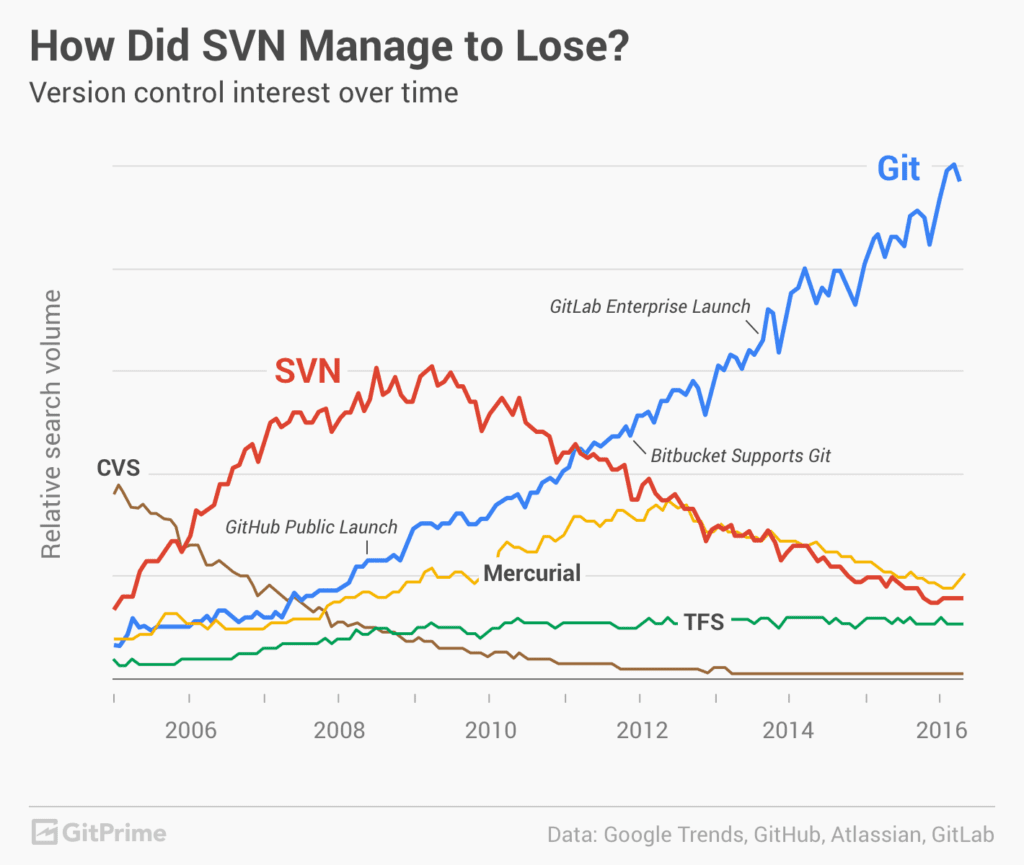
\includegraphics[frame,width=0.65\linewidth]{gitgraph.png}
    \captionof{figure}{Interés por los distintos sistemas de control de versiones. \href{https://fahadhussaincs.blogspot.com/2018/07/git-vs-github-understanding-and.html}{Fuente}.}
\end{center}

Wikipedia tiene una página donde se puede visualizar una \href{https://en.wikipedia.org/wiki/Comparison_of_version-control_software}{comparativa de distintos sistemas de control de versiones}. En ella se comparan información general, licencias, características, ... Es una buena manera de conocer otros sistemas aparte de los nombrados previamente.


\chapter{Características habituales}

Aunque cada sistema de control de versiones es diferente, todos tienen las siguientes características:

\begin{itemize}
    \item Comprobar el estado de los ficheros: si han sido modificados.
    \item Identificar cada cambio de una manera única.
    \item Conocer quién ha realizado las modificaciones que han sufrido los ficheros.
    \item Visualizar la diferencias que ha habido entre versiones en los ficheros.
    \item Volver atrás a una versión concreta del fichero, o de todo el proyecto.
    \item Tener un sistema de etiquetas para nombrar un estado concreto del proyecto.
\end{itemize}

Más adelante, con el ejemplo de Git, veremos qué significa cada una de esas características y cómo se realiza en Git.

\chapter{Tipos de sistemas de control de versiones}

Dentro de los sistemas de control de versiones se pueden diferenciar dos tipos cuando hablamos de cómo se interactúa y de cómo se almacena el histórico de todos los cambios.

\section{Centralizado}

El sistema centralizado era el más utilizado hasta la llegada y expansión de Git. Sistemas centralizados son CVS y Subversion.

El histórico de las modificaciones de nuestro repositorio se encontraba centralizado en un servidor. Cada vez que un usuario quería comprobar los cambios que había realizado, crear un commit, o volver a una versión anterior del proyecto \textbf{necesitaba realizar una conexión con el servidor central}.

\begin{center}
    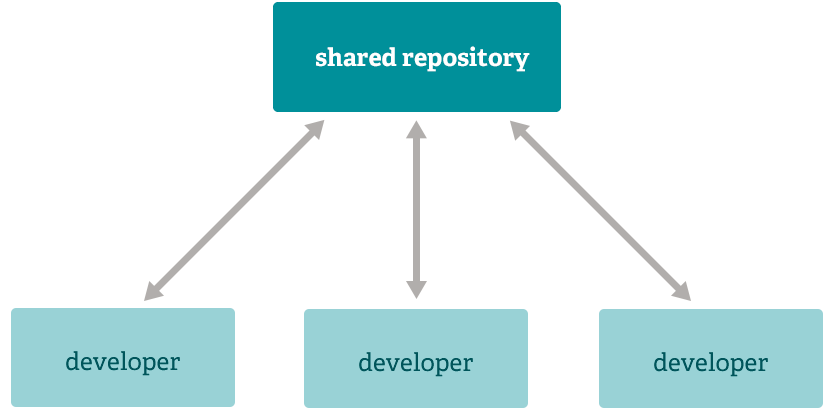
\includegraphics[width=0.65\linewidth]{workflow-a.png}
    \captionof{figure}{Arquitectura centralizada. \href{https://git-scm.com/about/distributed}{Fuente}.}
\end{center}

Esto suponía que era necesario tener siempre acceso a internet, y aparte, que para realizar pequeñas acciones cotidianas necesitases esperar a la respuesta del servidor.

Tampoco se podía saber si alguien había realizado modificaciones en el código hasta que no se intentasen subir nuevas modificaciones. De haber modificaciones y no tenerlas en la copia de trabajo local, había que resolver el conflicto, pudiendo dejar el servidor central en estado bloqueado.


\section{Distribuido}
Los sistemas de control de versiones distribuidos siguen la filosofía de que en cada copia de trabajo existen todos los datos, metadatos y el histórico completo de modificaciones que ha tenido el proyecto desde el inicio de los tiempos.

Gracias a eso, permite hacer uso del trabajo \textit{offline}, no necesitando la conexión a internet hasta que no nos interese subir los cambios realizados a un repositorio donde el resto de desarrolladores puedan acceder.

También es posible crear ramas locales, comprobar cómo ha evolucionado el proyecto, realizar \textit{diffs}... sin necesidad de realizar ningún tipo de conexión, por lo que estos cambios se realizan en local \textbf{mejorando la velocidad de trabajo}.

Trabajando de esta manera, también \textbf{nos permite centrarnos en las características que estamos realizando}, dejando para más adelante la posibilidad de que existan conflictos.

Por otro lado, el flujo de trabajo puede variar entre proyectos, y dentro de nuestro repositorio podemos tener distintos orígenes de los que obtener cambios. Un ejemplo de sistema distribuido:

\begin{center}
    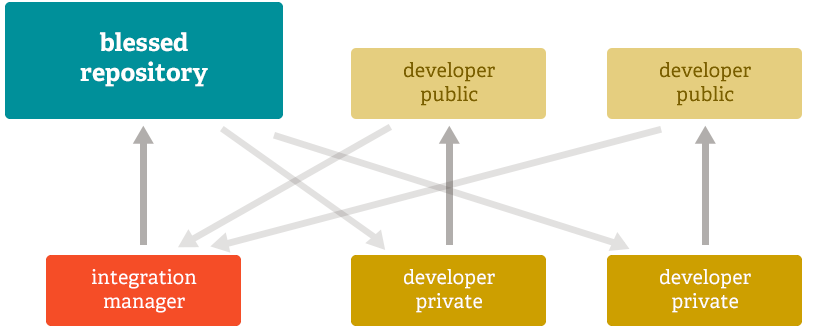
\includegraphics[width=0.65\linewidth]{workflow-b.png}
    \captionof{figure}{\textit{Workflow} distribuido. \href{https://git-scm.com/about/distributed}{Fuente}.}
\end{center}

En los sistemas distribuidos podemos hacer que el sistema de control de versiones se adapte a nuestra manera de trabajar, y no al revés.

\chapter{Glosario}
A la hora de utilizar un sistema de control de versiones tenemos que conocer cierta nomenclatura que es habitual. Es importante conocer estas palabras para identificar a qué términos nos estamos refiriendo.

Como son palabras utilizadas por los propios sistemas de control de versiones en sus clientes de línea de comandos (o en interfaces gráficas), se ha decidido mantener en inglés.


\begin{description}[style=nextline]
    \item[Blame] Comprobar el autor y la revisión de la última vez que se modificó una línea de un documento. En inglés \textit{blame} significa culpar/acusar.
    \item[Branch] Los sistemas de control de versiones nos permiten crear ramificaciones (temporales o perpetuas) partiendo de una versión concreta.
    \item[Checkout] Es utilizado para poner el repositorio local en una revisión concreta del histórico.
    \item[Clone] Clonar significa crear un repositorio obteniendo todas las revisiones de otro repositorio.
    \item[Commit] Puede tener dos acepciones:
    \begin{itemize}
        \item Como nombre: Un “\textbf{\textit{commit}}” (o revisión), es el conjunto de modificaciones que se empaquetan conjuntamente. Un “commit” muestra las modificaciones realizadas respecto al commit anterior.

        Los commits deberían llevar modificaciones que tengan que ver entre sí y tratando de que sea código válido.
        \item Como verbo: Hacer un “commit”, o “\textit{\textbf{commitear}}”, es la acción de empaquetar modificaciones de nuestra copia de trabajo, para crear un “\textit{commit}”, o revisión, que va a pertenecer al histórico del proyecto.
    \end{itemize}
    \item[Origin] En sistemas de control de versiones distribuidos, es el nombre del repositorio remoto “central”.
    \item[Pull] Obtener y aplicar en el repositorio local todos los commits desde un repositorio remoto.
    \item[Push] Enviar los commits creados en local que no están en el repositorio remoto “central”.
    \item[Repository] Puede tener distintas acepciones dependiendo del sistema de control de versiones que estemos utilizando. Es la estructura de directorios y ficheros (junto con su metadata) en el que guardamos el proyecto que nos interesa versionar. En sistemas distribuidos, tanto la copia local como la remota se denominan repositorios.
    \item[Tag] Una etiqueta es la manera de darle un nombre que podemos identificar de manera “humana” a una revisión concreta. Normalmente se usa para indicar las versiones del software: v1.0, v1.5, ...
    \item[Working copy] Es la copia local de un repositorio, en un momento específico del tiempo o revisión.
\end{description}
    \part{Introducción a Git}
    \chapter{Introducción}

\href{https://git-scm.com/}{Git} es un sistema de control de versiones distribuido creado en 2005 por Linus Torvalds, el mismo creador del kernel Linux. En tres días el sistema de control de versiones ya estaba versionando su propio código, y en dos semanas ya tenía gestión de ramas.

El proyecto se inició debido a que el sistema que utilizaban para la gestión del kernel Linux (Bitkeeper, en ese momento software privativo) decidió dejar de dar licencias gratuitas a los desarrolladores de Software Libre.

Linus hizo un análisis de los sistemas de control que existían en ese momento, y al ver que ninguno se adaptaba a las necesidades de un sistema tan complejo como el proyecto Linux, decidió crear uno propio.

Para el 16 de junio de 2005, Git manejaba el código fuente completo del kernel Linux, siendo el sistema utilizado a partir de ese momento. No sólo los cambios a partir de ese momento, si no que habían portado todo el histórico de cambios de los últimos 14 años.

\chapter{Características}

Git es un proyecto que ha crecido y ha añadido nuevas características, pero desde el inicio las más importantes fueron:

\begin{itemize}
    \item Sistema \textbf{distribuido}, por lo que cada desarrollador tiene una copia completa de todo el histórico y los cambios sin necesidad de necesitar acceso a internet.

    \item Compatible con los sistemas y protocolos actuales, como HTTPS, FTP y SSH.

    \item Debe permitir \textbf{desarrollos no lineales}, donde se permita crear ramas y unirlas de manera rápida y eficiente.

    \item \textbf{Eficiente} con proyectos grandes y gran cantidad de ficheros y desarrolladores. Al final, el propósito inicial era usarlo para el kernel Linux donde había miles de ficheros y desarrolladores.

    \item Los identificadores de los commits están basados en criptografía (SHA1). De esta manera no puedan existir dos commits con el mismo ID, y un ID representa única y exclusivamente un commit.
\end{itemize}


\chapter{Instalación}

Git está presente en todos los sistemas operativos actuales. Dependiendo del sistema operativo que utilicemos, podremos instalarlo de distintas maneras. En la  \href{https://git-scm.com/download/}{web oficial} están las últimas versiones.

Podemos hacer uso de Git a través de sistemas de consola o de aplicaciones gráficas. Hoy en día los entornos de desarrollo más conocidos también lo tienen integrado, por lo que es posible hacer uso de Git desde ellos.

\begin{itemize}
    \item Windows:
    \begin{itemize}
        \item \href{https://gitforwindows.org/}{Git Bash}
    \end{itemize}
    \item MacOS:
    \begin{itemize}
        \item MacOS tiene integrado Git dentro de las herramientas de desarrollador de Xcode. Para instalar únicamente Git desde un terminal debemos ejecutar:  \commandbox{xcode-select --install}
        \item Como mejor opción se recomienda usar \href{https://brew.sh/}{Brew.sh} e instalarlo a través de él.
    \end{itemize}
    \item GNU/Linux:
    \begin{itemize}
        \item Hoy en día todas las distribuciones tienen en sus repositorios Git, por lo que lo recomendable es hacer uso del sistema de instalación propio (apt, yast, ...). También es probable que ya esté instalado.
    \end{itemize}
\end{itemize}


\chapter{Primeros pasos}

Una vez instalado, debemos realizar una pequeña configuración que después se utilizará cada vez que realicemos un commit: crear una identidad.

\begin{mycode}{Añadiendo nuestro nombre y e-mail}{console}{}
ruben@vega:~$ git config --global user.name "Ruben Gomez"
ruben@vega:~$ git config --global user.email ruben@example.com
\end{mycode}

Esta configuración se guarda dentro de un fichero de configuración en la carpeta raíz de nuestro usuario. El fichero es \configfile{.gitconfig}. En este fichero podremos añadir configuraciones que se aplicarán a los comandos que realicemos.

A nivel de configuración podemos llegar a tener configuraciones específicas globales, del sistema, del repositorio y del área de trabajo, pero no entraremos en ello.

\chapter{Estado de los ficheros}
Dentro del repositorio, los ficheros que vayamos creando y/o modificando pueden estar en distintos estados. Esto es lo que se denomina “ciclo de vida” o \textit{lifecycle} de un fichero.Los ficheros pueden estar en los siguientes estados:

\begin{itemize}
    \item \textbf{Sin seguimiento}: Es un fichero nuevo que no está en seguimiento por el sistema de control de versiones. Aunque se realicen cambios en él, no podremos volver a versiones previas. En caso de usar un repositorio remoto, este fichero no estará en él.

    \item \textbf{Con seguimiento}: Estos ficheros pueden estar en los siguientes estados:
    \begin{itemize}
        \item \textbf{Sin modificar}: El fichero no ha sufrido modificaciones desde el último commit.
        \item \textbf{Modificado}: El fichero tiene modificaciones.
        \item \textbf{Preparado}: En inglés “staged”. Es un área donde se encuentran los ficheros que van a ir en el siguiente commit.
    \end{itemize}
\end{itemize}

En esta imagen se puede ver cómo los ficheros pueden cambiar de estado, y desde qué estado pasar a otro:

\begin{center}
    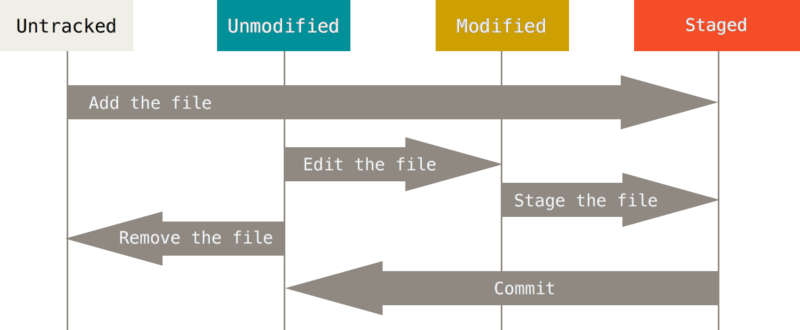
\includegraphics[width=0.9\linewidth]{lifecycle.png}
    \captionof{figure}{Estado de los ficheros. \href{https://git-scm.com/book/en/v2/Git-Basics-Recording-Changes-to-the-Repository}{Fuente}.}
\end{center}

Para entender esto mejor lo veremos a medida que vayamos haciendo uso de los comandos y creando/modificando ficheros.

\chapter{Comandos básicos}

Vamos a crear un repositorio para empezar a entender qué es lo que sucede con los ficheros que vamos creando en él, y tratar de entender los comandos más básicos.

\section{Crear repositorio local}

Vamos a crear un repositorio local dentro de un directorio nuevo, donde crearemos un proyecto que queremos versionar. Todo ello lo vamos a hacer dentro de un directorio nuevo llamado \configdir{pruebas}.

\begin{mycode}{Crear un repositorio git}{console}{}
ruben@vega:~$ mkdir pruebas
ruben@vega:~$ cd pruebas
ruben@vega:~/pruebas$ git init
Inicializado repositorio Git vacío en /home/ruben/pruebas/.git/

ruben@vega:~/pruebas$ ls -a
.  ..  .git/
\end{mycode}

Tal como se puede ver, ejecutando \commandbox{git init} dentro del directorio, nos inicializa el repositorio. Podemos ver que nos ha creado un directorio \configdir{.git}, que es un directorio oculto donde dentro se guarda la configuración y los commits que iremos realizando.

\errorbox{\textbf{No hagas cambios (ni borres nada) dentro del directorio .git}}


\section{Crear primer commit}

Con nuestro editor de textos favoritos, vamos a crear un fichero \configfile{README.md}. Normalmente este fichero es creado para indicar (en formato \href{https://es.wikipedia.org/wiki/Markdown}{Markdown}) información acerca del contenido del proyecto, qué es, para qué sirve, cómo compilarlo/usarlo...

Una vez creado el fichero vamos a entender qué es lo que está sucediendo dentro del repositorio:

\begin{mycode}{Comprobar estado del repositorio}{console}{}
ruben@vega:~/pruebas$ git status
En la rama main
No hay commits todavía

Archivos sin seguimiento:
(usa "git add <archivo>..." para incluirlo a lo que será confirmado)
README.md

no hay nada agregado al commit pero hay archivos sin seguimiento
presentes (usa "git add" para hacerles seguimiento)
\end{mycode}


Vemos que el estado del único fichero que hemos creado es “sin seguimiento” (tal como hemos explicado en el punto anterior). Es momento de pasar nuestro fichero a estado “preparado”, para ello:

\begin{mycode}{Preparamos el fichero para hacer commit}{console}{}
ruben@vega:~/pruebas$ git add README.md
ruben@vega:~/pruebas$ git status
En la rama main
No hay commits todavía

Cambios a ser confirmados:
(usa "git rm --cached <archivo>..." para sacar del área de stage)
nuevos archivos: README.md
\end{mycode}

El fichero \configfile{README.md} está en el área “stage”, por lo que ahora es el momento en el que podemos hacer nuestro primer commit con las modificaciones realizadas:


\begin{mycode}{Hacemos el commit}{console}{}
ruben@vega:~/pruebas$ git commit -m "Primer commit"
[main (commit-raíz) 45900ae] Primer commit
1 file changed, 3 insertions(+)
create mode 100644 README.md

guruben@vega:~/pruebas$ git status
En la rama main
nada para hacer commit, el árbol de trabajo está limpio
\end{mycode}

Con \commandbox{git commit -m “Primer commit”} lo que estamos es “encapsulando” todas las modificaciones de todos los ficheros que están en el área “stage” (en este caso un único fichero), y vamos a generar un commit al que le hemos puesto el mensaje “Primer commit”.


\section{Ver histórico de cambios}
Si realizamos varios cambios al fichero, o si añadimos un fichero nuevo y realizamos una serie de commits, nos puede interesar saber cómo está yendo el histórico de commits.

Para ello podemos hacer uso del comando \commandbox{git log}, que nos mostrará en orden por fecha descendente, todos los commits que ha tenido nuestro repositorio:

\begin{mycode}{Ver histórico de commits}{console}{}
ruben@vega:~/pruebas$ git log

commit ac00ce47dcdcda01bf33d162890bd98cc4f36ead (HEAD -> main)
Author: Rubén Gómez <ruben@example.com>
Date:   Sun Sep 17 10:52:26 2023 +0200

Añadir hola.java

commit a3f9554e0917dfdd2ce6ccccb5957d44d63c7f6f
Author: Rubén Gómez <ruben@examplel.com>
Date:   Sun Sep 17 10:52:03 2023 +0200

Añadir datos a README

commit 45900aef0300bf88c3a2939b8cf2f6b05de572dc
Author: Rubén Gómez <ruben@example.com>
Date:   Sun Sep 17 10:46:12 2023 +0200

Primer commit
\end{mycode}

De manera gráfica, el histórico de los \textit{commits} podríamos representarlo de la siguiente manera:

\begin{center}
    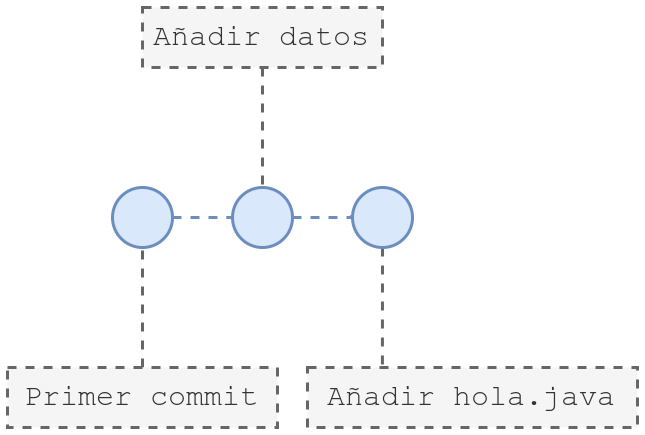
\includegraphics[width=0.6\linewidth]{log.png}
    \captionof{figure}{Estado tras varios commits}
\end{center}

    \part{GitHub como servidor remoto}
    \chapter{Usar GitHub como repositorio remoto}
\href{https://github.com/}{GitHub} es un portal donde podemos crear repositorios para poder usarlo como sistema centralizado de nuestros proyectos.

Entre las característica que tiene, se pueden destacar:
\begin{itemize}
    \item Entorno gráfico para controlar el repositorio. Se puede ver el histórico del repositorio, quién ha realizado los cambios, cuándo, ramas creadas...
    \item Control de incidencias. Para poder crear “\textit{issues}” del proyecto a medida que encontremos errores.
    \item Generar documentación por proyecto en formato Wiki.
    \item Gestión de “\textit{pull requests}” para integrar cambios en la rama principal.
    \item Sistema de “acciones”, que ayudan para el sistema de “integración continua”. Con estas acciones podemos generar “\textit{releases}”, compilar el código y comprobar si hay errores, pasar tests, ... Hay mucha \href{https://docs.github.com/en/actions}{documentación} al respecto.
\end{itemize}

\section{Crear repositorio}

Una vez hemos creado una cuenta, podremos crear un nuevo repositorio en la plataforma. Al crearlo, podemos elegir distintas configuraciones:

\begin{itemize}
    \item \textbf{Nombre del repositorio}, para poder acceder a él. Es recomendable darle un nombre significativo al proyecto.
    \item \textbf{Descripción}, donde podremos indicar un poco de texto para entender de qué trata el proyecto.
    \item \textbf{Visibilidad}. Podemos hacer que el repositorio sea \textbf{público} (cualquier persona puede ver el contenido del proyecto) o \textbf{privado} (sólo nuestro usuario puede verlo).

    \item \textbf{Inicializar el proyecto con}: Podemos hacer que cuando Github inicialice el proyecto le añada ciertos ficheros:
    \begin{itemize}
        \item \textbf{README}: Fichero donde indicar de qué trata el fichero, cómo compilarlo, ...
        \item \textbf{.gitignore}: Un fichero que nos permite ignorar ficheros dentro de nuestro “área de trabajo”. Podemos elegir de una plantilla para distintos lenguajes de programación.
        \item \textbf{Licencia}: Un fichero con distintas licencias libres para nuestro proyecto.
    \end{itemize}
\end{itemize}


\begin{center}
    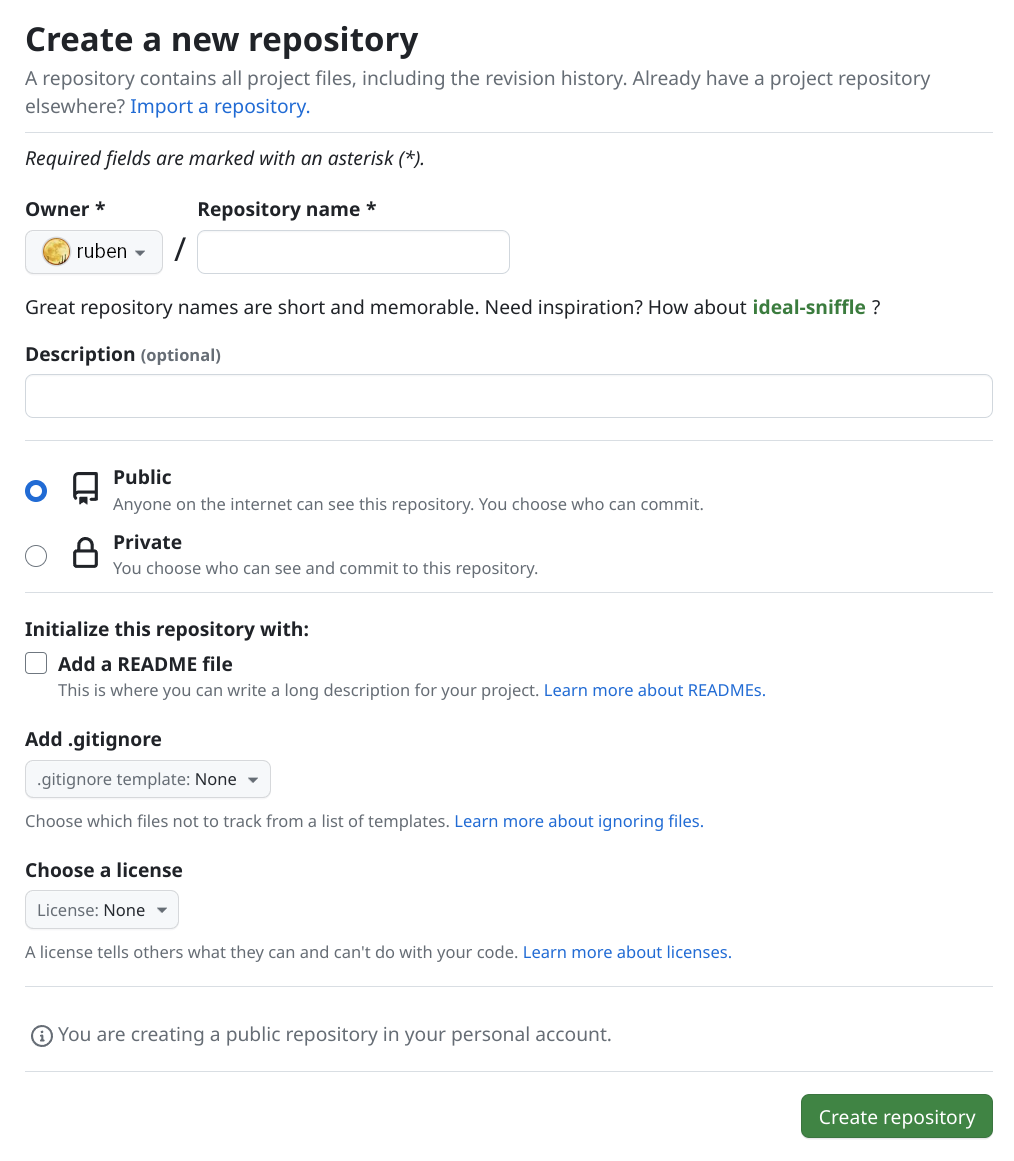
\includegraphics[frame,width=0.7\linewidth]{github-new.png}
    \captionof{figure}{Opciones al crear un nuevo repositorio en GitHub}
\end{center}

En este caso se va a crear un repositorio público llamado \textbf{pruebas}, sin ningún tipo de fichero. De esta manera “enlazaremos” el repositorio local de los pasos anteriores con este repositorio.


\chapter{Enlazar repositorio con remoto}

GitHub nos muestra cuáles son los pasos para enlazar un repositorio existente con el que acabamos de crear en su plataforma, a través de la línea de comandos:

\begin{mycode}{Enlazando repositorio local con uno en GitHub}{console}{{\small }}
ruben@vega:~/pruebas$ git remote add origin git@github.com:yuki/pruebas.git
ruben@vega:~/pruebas$ git branch -M main
ruben@vega:~/pruebas$ git push -u origin main
\end{mycode}

Vamos a tratar de entender qué es lo que hace cada uno de los comandos, ya que es importante.

\begin{itemize}
    \item \commandbox{git remote add origin git@github.com:yuki/pruebas.git}

    Con este comando se añade un repositorio remoto con el nombre “\textbf{origin}”. Básicamente estamos diciéndole al repositorio local que cuando realicemos algo sobre el repositorio remoto “origin” haga uso de esa URL.

    El nombre “origin” se puede cambiar, pero es el nombre que decidieron ponerle:

    \begin{center}
        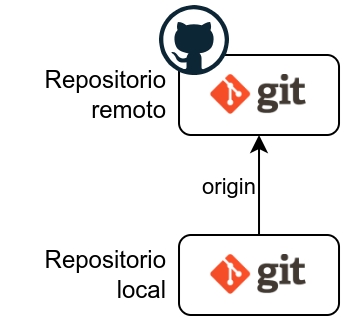
\includegraphics[width=0.7\linewidth]{remote.png}
        \captionof{figure}{Enlazamos repositorio local con remoto de nombre “origin”}
    \end{center}

    \item \commandbox{git branch -M main}

    Este comando lo que hace es cambiar el nombre de la rama principal para que se llame “\textbf{main}”. Originalmente la rama principal se llamaba “master”, pero en 2020 decidieron cambiarlo a “main”.

    En las nuevas versiones de git “main” ya es el nombre por defecto, por lo que este comando puede no ser necesario (si se ejecuta no hace nada).

    \item \commandbox{git push -u origin main}

    Este comando se puede separar en dos partes:
    \begin{itemize}
        \item \commandbox{git push}

        Este es el comando que utilizaremos para enviar al repositorio remoto los commits que hemos realizado en el repositorio local.

        \item \commandbox{-u origin main}

        Estos parámetros sólo los usaremos para realizar el primer envío. Estos indican al repositorio local que haga uso del servidor remoto “origin” para enlazar la rama en la que nos encontramos (“main”) con la rama remota “main” a la hora de enviar las revisiones.

        Los nombres de las ramas no tienen por qué coincidir, pero que sean iguales nos va a facilitar identificar ambas.

        \begin{center}
            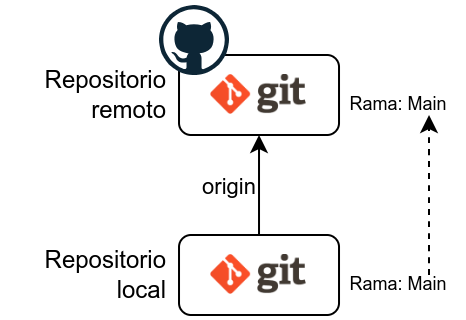
\includegraphics[width=0.7\linewidth]{remote_push.png}
            \captionof{figure}{Enlazamos rama local con rama remota}
        \end{center}
    \end{itemize}

\end{itemize}

Al realizar el último comando en windows nos aparecerá una ventana para que realicemos el \textbf{login de usuario} en GitHub.

\section{Añadiendo credenciales de acceso en Windows}

Dado que realizar una modificación en un repositorio de GitHub es algo que puede puede conllevar un peligro en el código fuente, nos aparecerá una ventana para que realicemos el login de usuario.

\begin{center}
    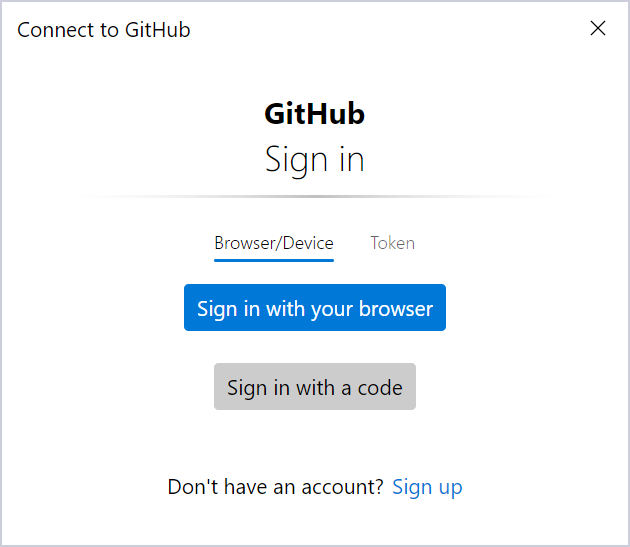
\includegraphics[frame,width=0.5\linewidth]{github_login.png}
    \captionof{figure}{Ventana para realizar el login en GitHub}
\end{center}

Elegiremos la opción marcada en azul, lo que nos abrirá el navegador web para realizar el login en la web de GitHub. Una vez hayamos introducido bien los credenciales de acceso, veremos la confirmación. Esto nos creará una autenticación “OAuth de aplicación” en \href{https://github.com/settings/applications}{nuestro perfil de GitHub} (Usuario → Settings → \href{https://github.com/settings/applications}{Applications}), pestaña “\textit{Authorized OAuth Apps}”.

\begin{center}
    
\includegraphics[frame,width=0.5\linewidth]{github_login2.png}
    \captionof{figure}{Login realizado correctamente}
\end{center}

Y para que siga funcionando, en el \textbf{Administrador de Credenciales} de Windows (“Panel de Control → Cuentas de Usuario → Administrador de Credenciales → Credenciales de Windows”), también nos creará una entrada nueva de credenciales genéricas:

\begin{center}
    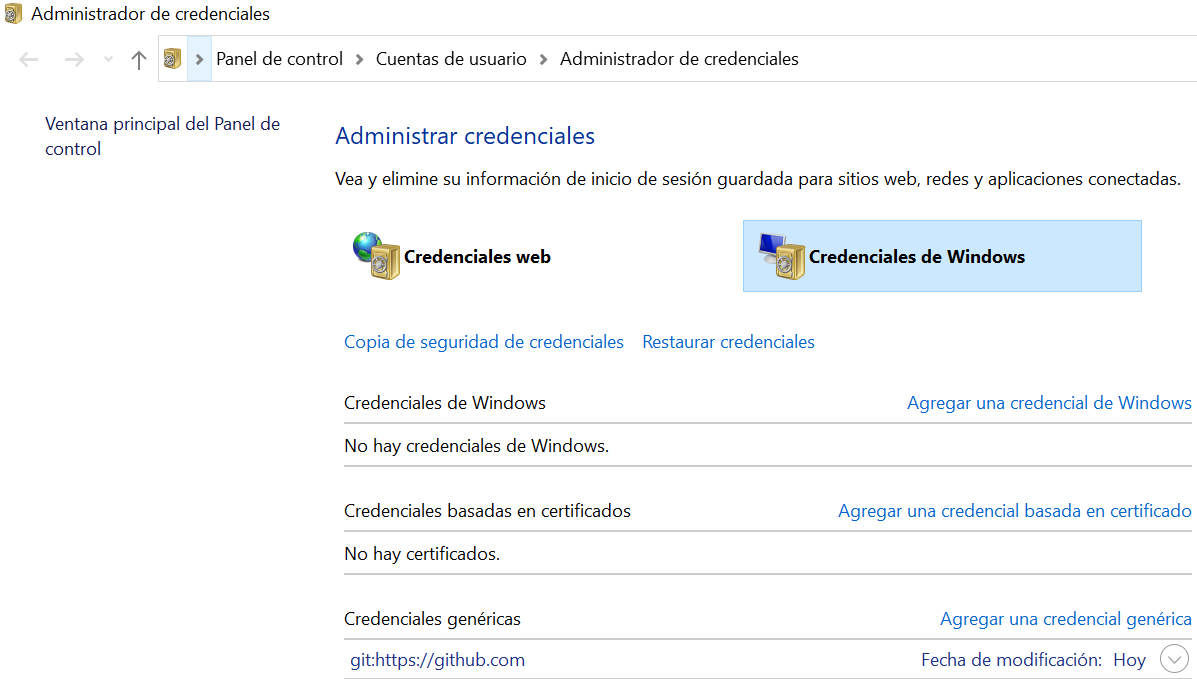
\includegraphics[frame,width=0.9\linewidth]{windows_credentials.png}
    \captionof{figure}{Credenciales de GitHub en Windows}
\end{center}

Una vez realizados estos pasos, nos funcionará el comando y enlazará la rama y enviará los commits realizados al servidor remoto.

\begin{mycode}{Enlazando la rama y enviando los cambios}{console}{}
ruben@vega:~/pruebas$ git push -u origin main
Enumerando objetos: 10, listo.
Contando objetos: 100% (10/10), listo.
Compresión delta usando hasta 6 hilos
Comprimiendo objetos: 100% (7/7), listo.
Escribiendo objetos: 100% (10/10), 889 bytes | 222.00 KiB/s, listo.
Total 10 (delta 2), reusados 0 (delta 0), pack-reusados 0
remote: Resolving deltas: 100% (2/2), done.
To github.com:yuki/pruebas.git
* [new branch]      main -> main
rama 'main' configurada para rastrear 'origin/main'.
\end{mycode}


\chapter{Enviar modificaciones locales}

A partir de ahora, cualquier modificación que hayamos realizado en local \textbf{deberemos enviarla al servidor remoto}. No tenemos por qué hacerlo por cada commit, ya que cuando realicemos el envío se enviarán todos los que no estén en remoto.

\begin{mycode}{Enlazando la rama y enviando los cambios}{console}{}
ruben@vega:~/pruebas$ git push
git push
Enumerando objetos: 5, listo.
Contando objetos: 100% (5/5), listo.
Compresión delta usando hasta 6 hilos
Comprimiendo objetos: 100% (3/3), listo.
Escribiendo objetos: 100% (3/3), 324 bytes | 324.00 KiB/s, listo.
Total 3 (delta 1), reusados 0 (delta 0), pack-reusados 0
remote: Resolving deltas: 100% (1/1), completed with 1 local object.
To github.com:yuki/pruebas.git
cefb314..2cac944  main -> main
\end{mycode}


\chapter{Clonar repositorio remoto}

Imaginemos que una vez subido los cambios locales a GitHub queremos hacer uso del repositorio en otro ordenador. Para ello, debemos realizar un “clonado” del repositorio en cuestión.

\begin{mycode}{Clonar repositorio remoto en repositorio local}{console}{}
ruben@vega:~/pruebas$ git clone https://github.com/yuki/pruebas.git
Clonando en 'pruebas'...
remote: Enumerating objects: 20, done.
remote: Counting objects: 100% (20/20), done.
remote: Compressing objects: 100% (12/12), done.
remote: Total 20 (delta 4), reused 20 (delta 4), pack-reused 0
Recibiendo objetos: 100% (20/20), listo.
Resolviendo deltas: 100% (4/4), listo.
\end{mycode}


\chapter{Obtener últimos commits}

Si alguien ha realizado commits en nuestro repositorio (o los hemos realizado nosotros desde otro ordenador), es posible que nuestro repositorio local no esté actualizado. Para actualizarlo tenemos que entender dos comandos:

\begin{itemize}
    \item \commandbox{git fetch}

    Obtiene los commits del repositorio remoto, \textbf{pero no los aplica sobre nuestra copia de trabajo actual}. De esta manera, no se aplican los cambios y mientras tanto podemos seguir trabajando.

\begin{mycode}{Titulo}{console}{}
ruben@vega:~/pruebas$ git fetch
remote: Enumerating objects: 5, done.
remote: Counting objects: 100% (5/5), done.
remote: Compressing objects: 100% (3/3), done.
remote: Total 3 (delta 0), reused 3 (delta 0), pack-reused 0
Desempaquetando objetos: 100% (3/3), 326 bytes | 27.00 KiB/s, listo.
Desde github.com:yuki/pruebas
2cac944..97f5359  main       -> origin/main

ruben@vega:~/pruebas$ git status
En la rama main
Tu rama está detrás de 'origin/main' por 1 commit, y puede ser
avanzada rápido. (usa "git pull" para actualizar tu rama local)
\end{mycode}

    Tal como se puede ver el primer comando nos descarga objetos nuevos, y al ver el estado nos avisa que \textbf{nuestra rama está por detrás de “origin/main”} (la rama remota). También podemos ver todos los commits de la siguiente manera:

\begin{mycode}{Titulo}{console}{}
ruben@vega:~/pruebas$ git log --all
commit 97f5359058551cfbe1d61c7b3db1bd648ac496ba (origin/main)
Author: Rubén Gómez <pruebas@example.com>
Date:   Sun Sep 17 19:40:18 2023 +0200

Pequeño cambio en el README

commit 2cac94467ca7c50e2cf2125ce11e21eda8461cc1 (HEAD -> main)
Author: Rubén Gómez <pruebas@example.com>
Date:   Sun Sep 17 18:40:37 2023 +0200

Añadiendo “adios” en hola.java

commit cefb3143e3f298dc8fe200d6a2804165f58bab69
Author: Rubén Gómez <pruebas@example.com>
Date:   Sun Sep 17 18:40:02 2023 +0200

Corregido error en hola.java
\end{mycode}

    El primer commit nos indica que está en \textbf{origin/main}, la rama del repositorio remoto, mientras que el segundo  nos aparece “\textbf{\texttt{HEAD -> \ main}}”, que es la copia de trabajo local. El resumen sería:

    \begin{center}
        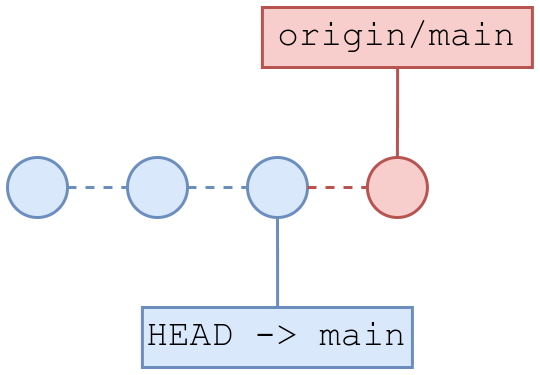
\includegraphics[width=0.5\linewidth]{fetch.png}
        \captionof{figure}{Estado de los commits tras el “fetch”}
    \end{center}


    \item \commandbox{git pull}

    En este caso se obtienen los commits del repositorio \textbf{y se aplican sobre la rama de trabajo actual}. Si tenemos cambios realizados en local, los cambios que obtenemos del repositorio \textbf{pueden entrar en conflicto con lo que tenemos}. Más adelante hablaremos de ello.

    De no existir conflictos, los cambios se aplican y el estado quedaría en ambos repositorios en el mismo punto exacto:

    \begin{center}
        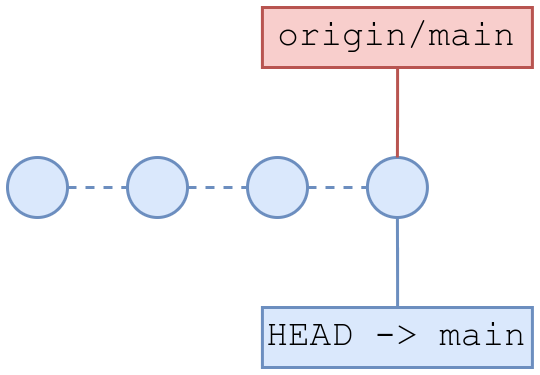
\includegraphics[width=0.5\linewidth]{pull.png}
        \captionof{figure}{Estado de los commits tras el “pull”}
    \end{center}
\end{itemize}



    \part{Ramas, \textit{merges} y conflictos}
    \chapter{Usar ramas en git}

La creación de ramas (llamadas \textbf{\textit{branches}}) en un repositorio nos permite realizar pruebas, añadir características nuevas, o cambiar de ámbito sin perjudicar el flujo de trabajo principal.

Una rama es una bifurcación del camino principal del desarrollo de una aplicación (o de un commit concreto). Esta rama puede ser una rama pública (existir en GitHub) o ser privada (sólo existir en nuestro repositorio local).

La creación de ramas en Git es instantáneo (al contrario de lo que sucedía con sistemas anteriores), por lo que crearla no supone un esfuerzo ni una pérdida de tiempo para el desarrollo.

\begin{center}
    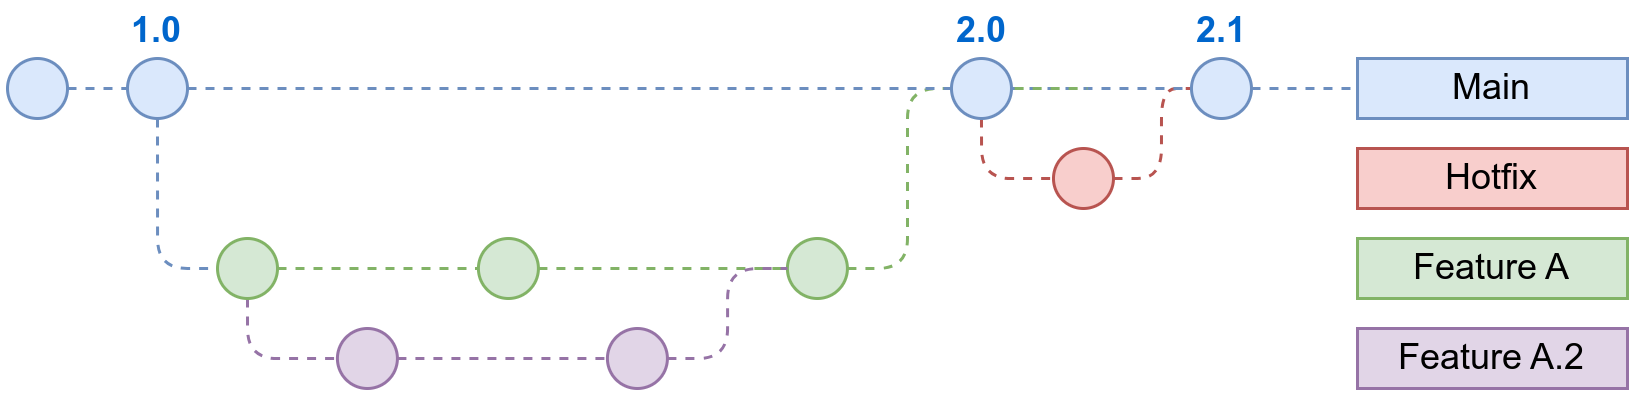
\includegraphics[width=0.9\linewidth]{ramas.png}
    \captionof{figure}{Un desarrollo con ramas}
\end{center}

En el dibujo aparecen ramas que posteriormente se unen a la rama \textit{main} principal, pero esto no tiene por qué ser así, y una rama puede mantener un desarrollo paralelo y nunca unirse.

\section{Crear rama}
Para crear una rama en el desarrollo, desde el punto en el que nos encontramos, se puede hacer de dos maneras. El resultado es el mismo, pero conviene entender qué es lo que sucede en ambos casos.

\begin{itemize}
    \item \textbf{Crear rama y luego movernos a ella}: Este caso consta de dos pasos.

\begin{mycode}{Crear rama “featureA” y movernos a ella}{console}{}
ruben@vega:~/pruebas$ git branch featureA
ruben@vega:~/pruebas$ git checkout featureA
Cambiado a rama 'feature1'

ruben@vega:~/pruebas$ git log
commit 170f9ce8c214b82f... (HEAD -> featureA, origin/main, main)
Author: Rubén Gómez <ruben@example.com>
Date:   Sun Sep 17 18:40:37 2023 +0200
...
\end{mycode}

    Tal como se puede ver, se ha creado la rama con nombre “featureA”, para posteriormente con el comando \commandbox{git checkout featureA} cambiarnos a dicha rama.

    Con \commandbox{git log} podemos comprobar cómo en ese \textit{commit} ahora mismo se encuentran tres puntos de nuestro sistema de repositorios:
    \begin{itemize}
        \item \texttt{\textbf{HEAD -> featureA}}: que es la rama en la que nos encontramos ahora.
        \item \textbf{origin/main}: la rama “main” del repositorio remoto.
        \item \textbf{main}: la rama local “main”.
    \end{itemize}

    Los tres puntos coinciden porque no se han realizado todavía ningún cambio en ninguna rama.

    \item \textbf{Crear rama y movernos a ella automáticamente}: en este caso los dos pasos se convierten en uno, pero el resultado es el mismo.

\begin{mycode}{Crear rama “featureB” y movernos a ella directamente}{console}{}
ruben@vega:~/pruebas$ git checkout -b featureB
Cambiado a nueva rama 'featureB'
\end{mycode}
\end{itemize}

\section{Cambiar entre ramas}

Ahora que ya sabemos cómo crear ramas, hay que entender cómo podemos cambiar entre ellas, aunque el comando lo acabamos de ver en el punto anterior: \commandbox{git checkout branch}, donde “branch” es el nombre de la rama a la que queremos ir.

Siguiendo con el ejemplo anterior, si queremos volver a la rama “main”, deberíamos hacer:

\begin{mycode}{Volver a la rama “main”}{console}{}
ruben@vega:~/pruebas$ git checkout main
Cambiado a rama 'main'
Tu rama está actualizada con 'origin/main'.
\end{mycode}

Si queremos volver a la rama “featureA”:

\begin{mycode}{Volver a la rama “featureA”}{console}{}
ruben@vega:~/pruebas$ git checkout featureA
Cambiado a rama 'featureA'
\end{mycode}

\section{Ver estado de las ramas}

Para comprobar cuál es el estado de las ramas, vamos a realizar dos \textit{commits} distintos en la rama “main” y otro en la rama “featureA”. Para ver cómo se encuentra ahora el estado de nuestro repositorio, podemos hacer uso del siguiente comando:

\begin{mycode}{Volver a la rama “featureA”}{console}{{\footnotesize }}
$ git log --graph --all --pretty=format:'%Cred%h%Creset -%C(auto)%d%Creset %s  %Creset'
\end{mycode}

Obtendríamos el siguiente resultado:

\begin{center}
    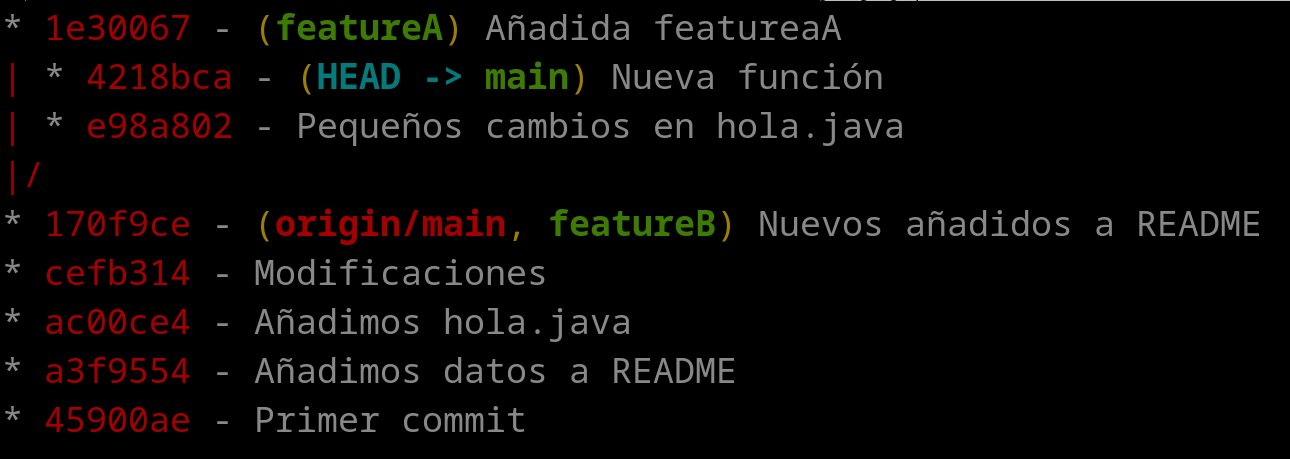
\includegraphics[width=0.9\linewidth]{ramas2.png}
    \captionof{figure}{Ramas actuales}
\end{center}

Tal como se puede ver, la bifurcación sucede en el commit “170f9ce”, que es donde está situado el último commit del servidor remoto y la rama “featureB” creada previamente (y que no se ha tocado).

Por otro lado, desde ese punto surgen dos ramas:
\begin{itemize}
    \item \textbf{featureA}, con el único commit 1e30067.
    \item \textbf{main}, que tiene 2 commits.
\end{itemize}

Tras realizar estas modificaciones, a continuación vamos a ver cómo podemos fusionar los cambios de una rama en la otra.


\chapter{Fusionar ramas}

La fusión de ramas (en inglés \textit{\textbf{merge}}) sucede cuando queremos obtener los cambios realizados en una rama y fusionar dichos cambios con la rama en la que nos encontramos actualmente.  Ahora que tenemos distintas ramas creadas, con sus correspondientes commits, es buen momento para realizar la fusión de las ramas.

Dependiendo de cómo haya sido el desarrollo de las ramas, la fusión podrá terminar en un “dibujo” distinto. Por ejemplo, el caso más sencillo es que en la bifurcación sólo la rama nueva tiene nuevos commits, por lo que al realizar la fusión quedaría:


\begin{center}
    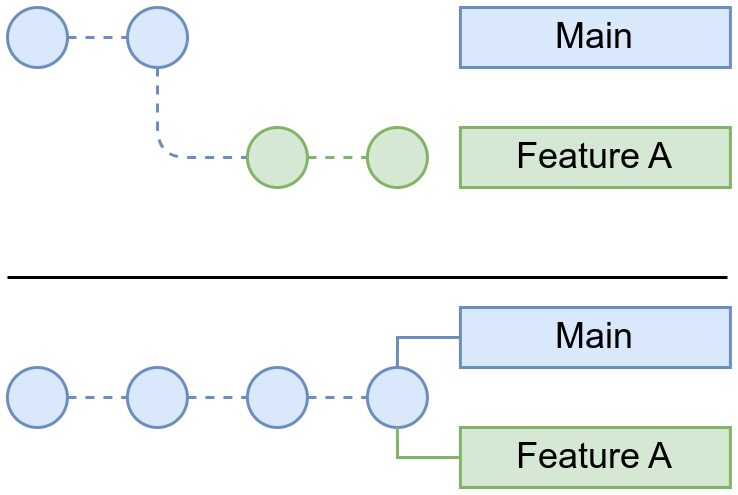
\includegraphics[width=0.6\linewidth]{merge_facil.png}
    \captionof{figure}{Merge de rama con commits sobre rama “main”}
\end{center}

Tras realizar el merge, en este caso es como si la rama “FeatureA”no hubiese existido.

En cambio, si en la rama main, tal como se ha sugerido en el punto anterior, también se realizan modificaciones, el dibujo quedará tal que así:

\begin{center}
    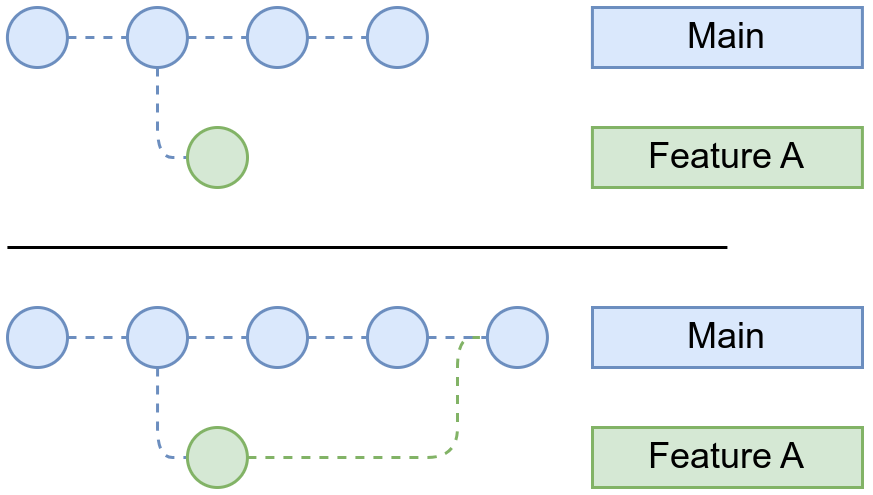
\includegraphics[width=0.6\linewidth]{merge_serio.png}
    \captionof{figure}{Merge donde hay commits en ambas ramas}
\end{center}


Para realizar la fusión, debemos seguir estos pasos:
\begin{itemize}
    \item Colocarnos en la rama en la que queremos fusionar los cambios de otra rama. Normalmente, nos va a interesar añadir los cambios a la rama “main”.
    \item Realizar la fusión.
\end{itemize}


\begin{mycode}{Volver a la rama “main”}{console}{}
ruben@vega:~/pruebas$ git checkout main
ruben@vega:~/pruebas$ git merge featureA -m "Merge de FeatureA en main"
\end{mycode}

De esta manera, crearemos un nuevo commit con el texto “Merge de FeatureA en main”, que indicará la fusión de la rama “featureA” sobre la rama Main. El dibujo en la vida real queda de la siguiente manera:


\begin{center}
    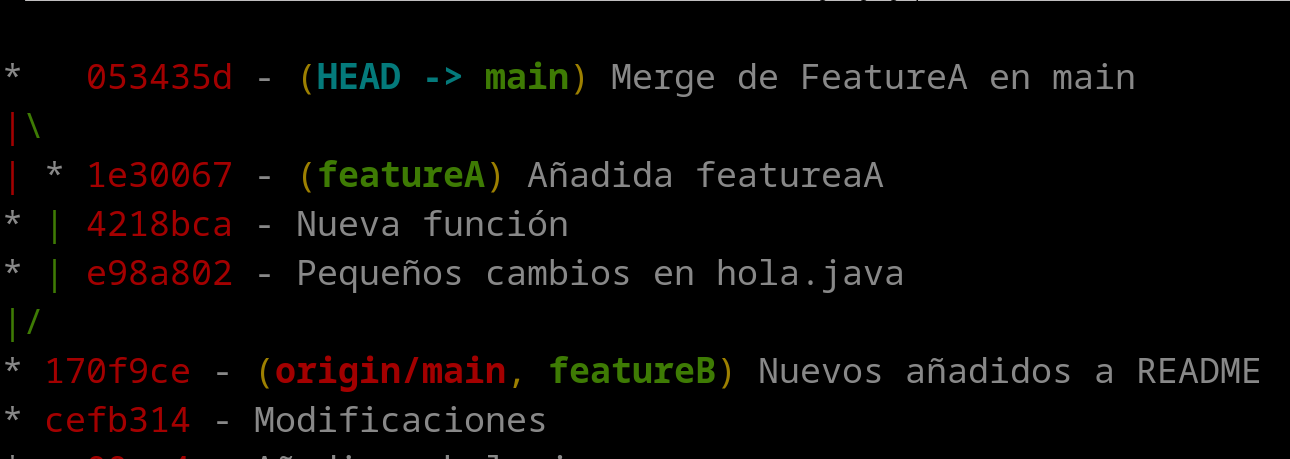
\includegraphics[width=0.9\linewidth]{merge_final.png}
    \captionof{figure}{Merge donde hay commits en ambas ramas}
\end{center}

Una vez realizado el \textit{merge}, podemos subir los cambios al repositorio central. La rama “featuresA” es una rama local, por lo que a nivel de GitHub esa rama nunca ha existido, aunque podemos ver en el interfaz web que el gráfico sí ha sufrido una ramificación:

\begin{center}
    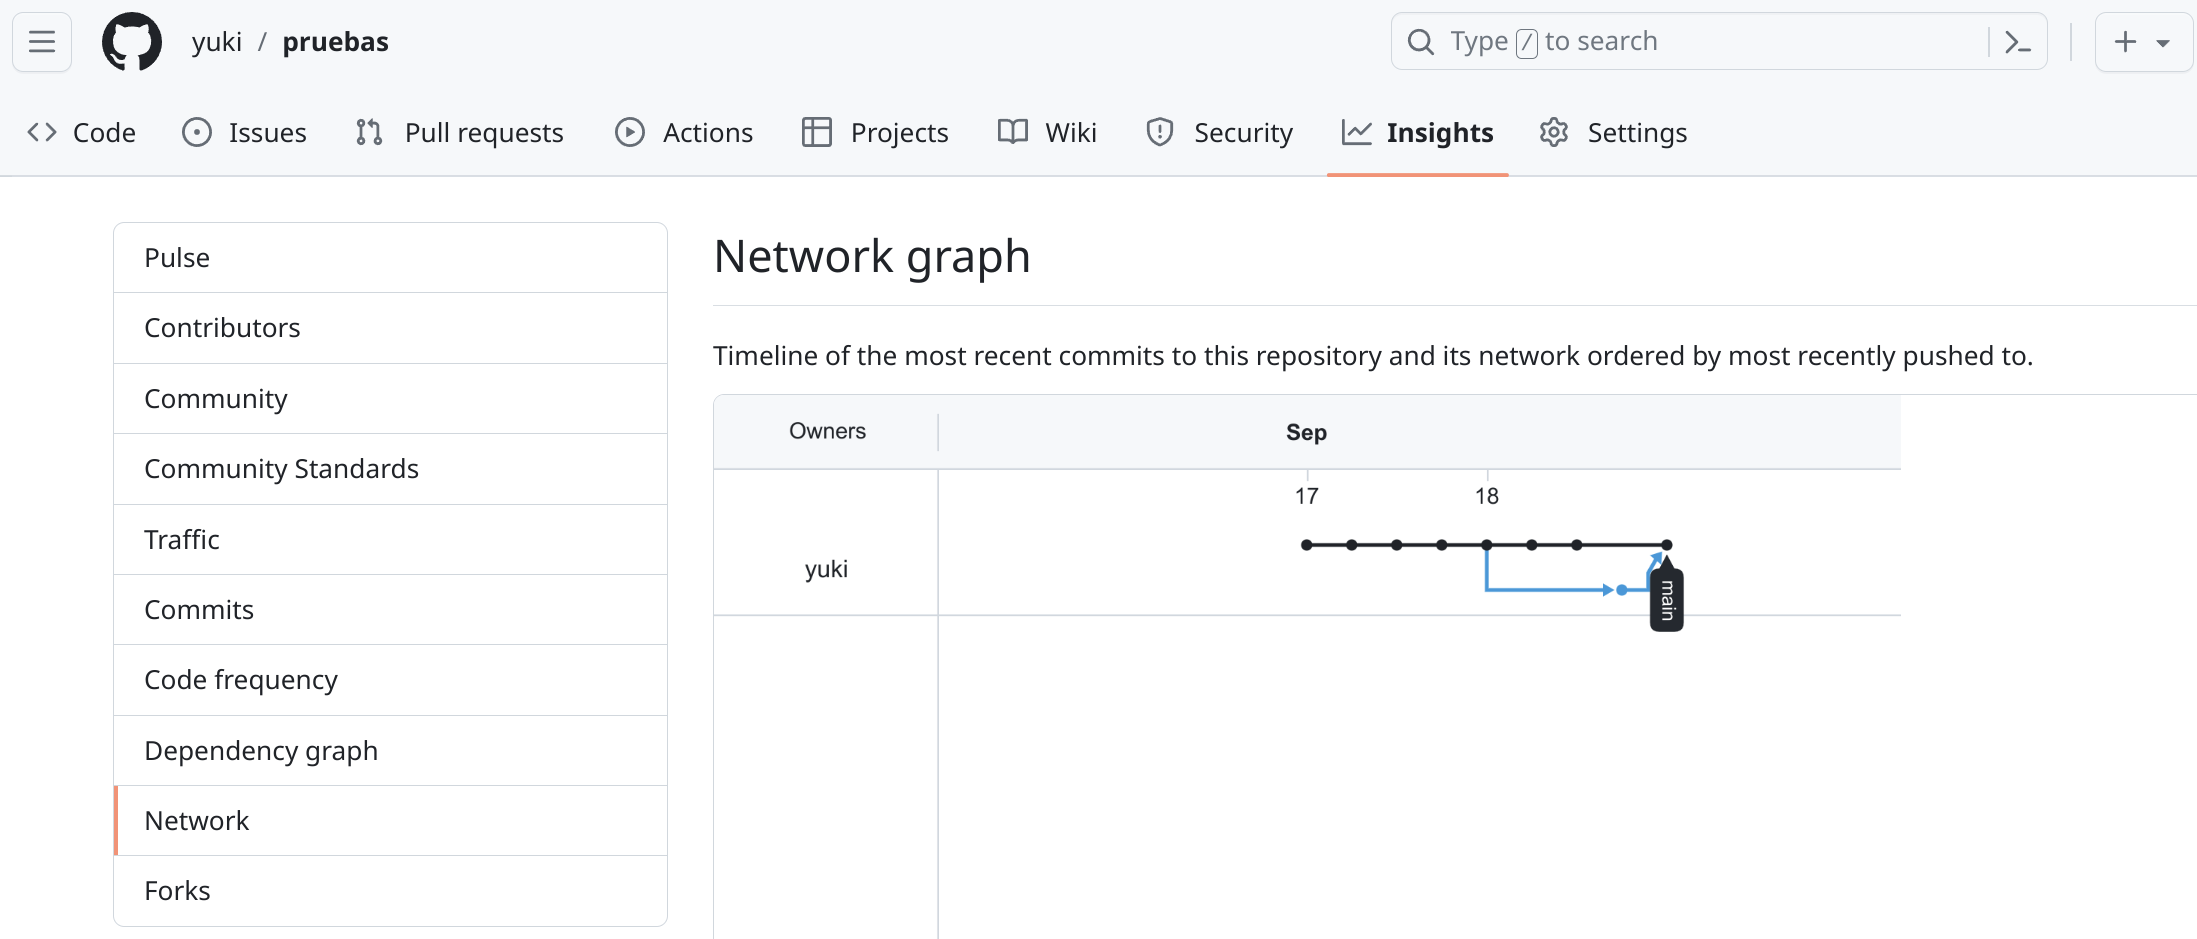
\includegraphics[frame,width=0.9\linewidth]{merge_github.png}
    \captionof{figure}{Gráfico en el interfaz de GitHub}
\end{center}

%    \part{Git y SSH}
%    explicar cómo funcion SSH con GitHub

%    \part{Configuraciones}
%    \input{5_configs.tex}
% .gitconfig
% .gitignore

%    \part{Git avanzado}
%    cherry-pick, hooks, pull requests

%    \part{GitHub actions}
%    crear algo del estilo github pages en HTML con la documentación del programa hecha con javadoc/doxygen

%    \graphicspath{{../../yukibook.cls/}}
%    \licensepage

\end{document}